\subsection{Memória}
A memória é a capacidade de adquirir, armazenar e recuperar informação. essa é uma definição que serve tanto para o meio biológico como para o meio artificial, podemos dizer que a memória  é tão importante quanto o processador e que é um dos principais componentes do computador. 
Com a função de armazenar a informação antes dela seguir para o processador a memória segue uma topologia que define sua utilização pelo SO, as camadas superiores têm uma velocidade mais alta, capacidade menor e um custo maior, o que se altera nas camadas inferiores que têm velocidade mais baixa, capacidade maior e um menor custo.
\begin{figure}[htpb]
    \centering
   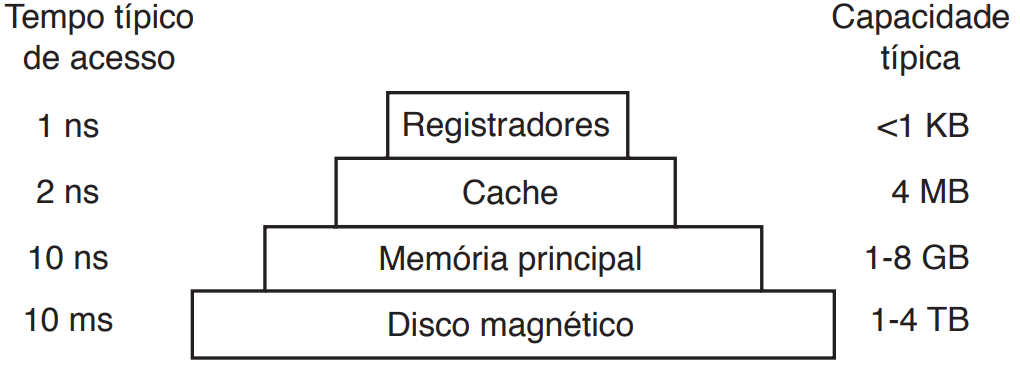
\includegraphics[scale=0.5]{imagens/lvlmemoria.png}
   \caption{Uma hierarquia de memória típica. Os números são apenas aproximações. \cite{Tanenbaum2016}}
   \label{fig:lvlmemoria}
\end{figure}\\

Na camada superior temos os registradores que são feitos do mesmo material do processador e possuem velocidade similar a deles, posteriormente temos o Cache que é principalmente controlada pelo hardware e pode se separar em até  três níveis cada nível  mais lento e maior que o anterior. O cache é erroneamente confundido com o buffer do processador mas basicamente ele tem por função servir como um espaço para informação de rápido acesso por exemplo  o cache L1 é dividido em memória de instrução e memória para dados. Com isso, o processador vai direto à memória de instrução, se estiver buscando uma instrução, ou vai direto à memória de dados, se estiver buscando um dado o cache L2 possui uma capacidade de armazenamento maior e é um pouco mais lento que o L1 ele serve para armazenar as informações antes delas irem para o cache L1 e assim sucessivamente o cache L3 diferente dos anteriores normalmente se apresenta fora do núcleo do processador e é compartilhado pelos núcleos como podemos ver na figura \ref{fig:cache} .
\begin{figure}[htpb]
    \centering
   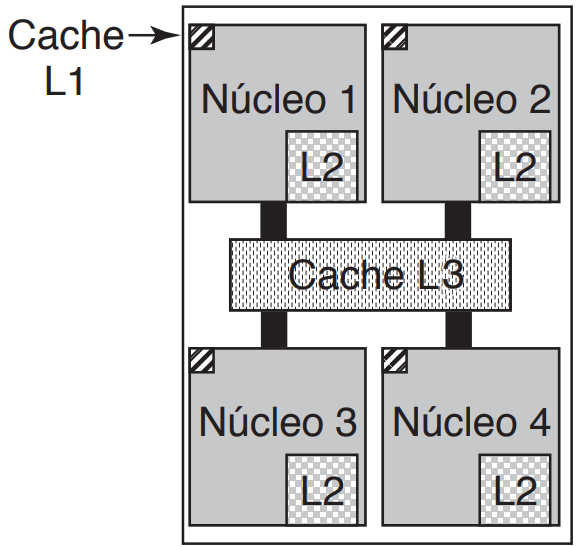
\includegraphics[scale=0.4]{imagens/cache.png}
   \caption{As memorias cache em um processador moderno.}
   \label{fig:cache}
\end{figure}\\

Logo em seguida vem a memória RAM (Random Access Memory — em portugues memória de acesso aleatório)Todas as requisições da CPU que não podem ser atendidas pela cache vão para a memória principal. Essa memória é responsável por realizar a leitura dos conteúdos quando requeridos, ou seja, de forma não-sequencial e guardar a informação de forma rápida para que seja lida cache assim como manter informações da cache.
\begin{figure}[htpb]
    \centering
   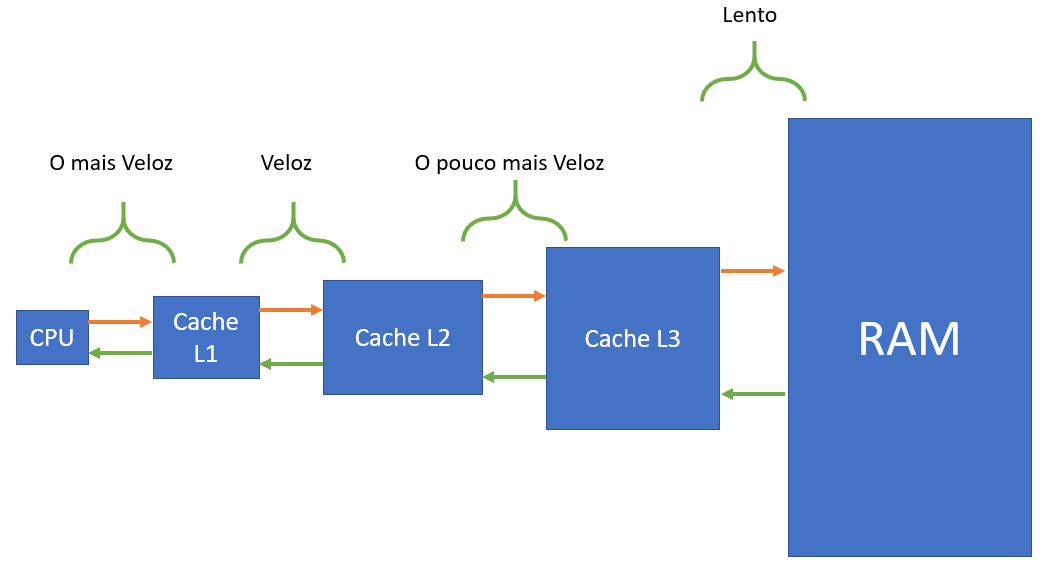
\includegraphics[scale=0.25]{imagens/velocidaderam.png}
   \caption{Do processador a RAM.}
   \label{fig:velocidade}
\end{figure}\\

A ROM (Read Only Memory — em portugues memória somente de leitura) é programada na fábrica e não pode ser modificada depois. Ela é rápida e barata. Em alguns computadores, o carregador (bootstrap loader) usado para inicializar o computador está contido na ROM.\\
A EEPROM (Electrically Erasable PROM — em portugues ROM eletricamente apagável) e a memória flash também são não voláteis, mas, diferentemente da ROM, podem ser apagadas e reescritas. No entanto, escrevê-las leva muito mais tempo do que escrever em RAM, então elas são usadas da mesma maneira que a ROM, apenas com a característica adicional de que é possível agora corrigir erros nos programas que elas armazenam mediante sua regravação. \\
A memória flash é um tipo particular de EEPROM que vem se tornando popular e  bastante comum e sendo utilizada fortemente em equipamentos portáteis. Utilizada em dispositivos como câmeras  e reprodutores de música substitui o disco rígido por manter as informações mesmo quando não está conectado diretamente a energia. Podemos dizer que a memoria flash esta entre a memora RAM e o discos rigidos no quesito velocidade. \\
A CMOS (Complementary Metal Oxide Semiconductor - em portugues 
Semicondutor de óxido de metal complementar
) é uma memória volátil e muito utilizada para armazenar a data e hora em sistemas, ela normalmente é alimentada por uma pequena bateria e seu consumo é tão baixo que a bateria que  é colocada de fábrica pode durar anos. Ela armazena informações básicas do sistema como data e hora ou por exemplo qual disco deve ser iniciado primeiro para iniciar o sistema operacional.
